\documentclass{standalone}
\usepackage{tikz}
\usepackage{ctex,siunitx}
\usepackage{tkz-euclide}
\usepackage{amsmath}
\usetikzlibrary{patterns, calc}
\usetikzlibrary {decorations.pathmorphing, decorations.pathreplacing, decorations.shapes,}
\begin{document}
\small
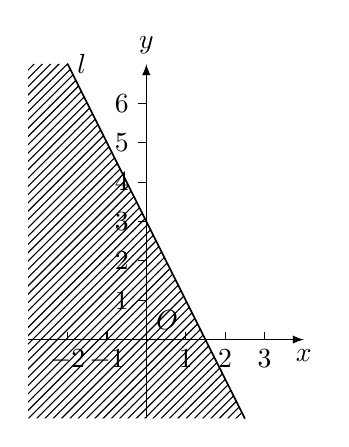
\begin{tikzpicture}[>=latex,scale=0.5]
  \draw[thin,->](-3,0)--(4.0,0)node[below]{$x$};
  \draw[thin,->](0,-2)--(0,7)node[above]{$y$};
  \tkzDefPoints{0/0/O,-2/7/M,2.5/-2/N,-3/7/P,-3/-2/Q}
  \foreach \x in {-2,-1,1,2,3}
  {
    \draw[thin](\x,0)--++(0,0.2)node[at start,below]{$\x$};
  }
  \foreach \x in {1,...,6}
  {
    \draw[thin](0,\x)--++(-0.2,0)node[left]{$\x$};
  }
  % \draw[densely dashed](1,-2)--(1,7);
  \tkzDrawLine[semithick,add= 0 and 0](N,M)
  \tkzLabelLine[pos= 1.0,right](N,M){$l$}
  \fill[pattern=north east lines](N)--(M)--(P)--(Q);
  % \tkzLabelPoints[right](A,B',C')
  % \tkzLabelPoints[left](B,C)
  % \tkzDrawPoints[fill=black](A,B,C,B',C')
  \tkzLabelPoints[above right](O)
\end{tikzpicture}
\end{document}